\scanpage{73}
% archive foliation: 72
[Ici, on montre que \inserted{la condition a) implique que}
pour $\forall X$ fixé, l'expression de a),
$G(f,g)=R(f,f',\ldots,f^{(n)};g,g',\ldots,g^{(n)})$ doit avoir
des coefficients $\in\mathbb{C}$, \unsure{indépendante|indépendants} de $X$, donc
\[
R\in\mathbb{C}(F_0,F_1,\ldots,F_n;G_0,\ldots,G_n)
\]
et en fait,
\[
R(\quad)=
\underbrace{P(F_0,\ldots;G_0,\ldots)}_{\in\mathbb{C}[F_0,\ldots,G_n]}
/F_1^pG_1^q
\]
]

On peut prendre
\[
G(f,g)=\bigl(
\left[-2\frac{g'''}{g'}+3\left(\frac{g''}{g'}\right)^2\right]
-\left[-2\frac{f'''}{f'}+3\left(\frac{f''}{f'}\right)^2\right]
dt^2
\]

De plus, on trouve un torseur canonique $\mathcal{T}_X$ \unsure{sous}
$\underline{\omega}_{X/\mathbb{C}}^{\otimes2}$,
dépend \unsure{fonctiellement|fonctoriellement} de $X$ (pour morphismes
étales), et
\[
\deleted{\unsure{\varphi}}\ c^X:\mathcal{P}_X\longrightarrow\mathcal{T}_X
\]
tel que
\[
\left\{\begin{array}{l}
G(f,g)=c^X(g)-c^X(f)\\
c^X\text{ se factorise en }H\backslash\mathcal{P}_X\longrightarrow\mathcal{T}_X\\
\text{ce dernier morphisme est un iso}
\end{array}\right.
\]

III) On prend maintenant $X$ \inserted{schémas} variable lisse
(\unsure{en} \unsure{gardant|grandes} diff. \unsure{lim.} à l'ordre $2$)
sur des schémas variables, et on cherche pour tt tel $X$
\diagram{\begin{tikzcd}
\mathcal{E}_X\times\mathcal{E}_X \arrow[r,"G"] & \omega_{X/S}^{2}
\end{tikzcd}}
de façon compatible aux chgt de base $S'\longrightarrow S$,
aux morphismes étales
\diagram{\begin{tikzcd}
X' \arrow[r] \arrow[dr,no head] & X \arrow[d,no head]\\
& S
\end{tikzcd}}
et satisfaisant aux conditions qui correspondent à a), b), c),
(\uline{plus} la condition d) \deleted{\unsure{e)}}
\inserted{si \deleted{\unsure{on}} $S$ corps de car. $0$, et e) dans}
\deleted{``\unsure{formulation possible} analytique complexe''}.

\margin{la \unsure{forme suivante}:
$G(f,g)$ \unsure{non identiquement|non ident.}
nul en \unsure{car.} $\unsure{p>0}$.}
\figure{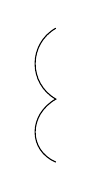
\begin{tikzpicture}
\draw (0,1.7) .. controls (-0.35,1.5) and (-0.35,1.0) .. (0,0.8)
.. controls (-0.35,0.6) and (-0.35,0.15) .. (0,0);
\end{tikzpicture}}

Mais quand on parle ``d'op. différentiel'', il faut maintenant remplacer
un polynôme $R$ en $f,f',f'',\ldots,g,g',g'',g'''$ par un
polynôme en
$f,f'=D_t^{(1)}f,D_t^{(2)}(f)\ldots D_t^{(n)}f,
g,g'=D_t^{(1)}g,D_t^{(2)}g,\ldots D_t^{(n)}g$.
\unsure{On voit clairement} à priori, les coeff.
sont dans $\Gamma(U,\underline{\mathcal{O}}_U)$
(où $t$, l'uniformisant, est défini sur $U$)
mais si on \deleted{\unsure{f}} en fait varier $X$, on
voit que les coefficients doivent être dans \uline{$\mathbb{Z}$}
(ou dans $\Gamma(S_0,\mathcal{O}_{S_0})$ si on a fixé un schéma de base
commun $S_0$ pour les $S,X\ldots$).
On trouve encore l'existence d'un tel, et l'unicité
à un facteur $\varepsilon\in\mathbb{Z}^{*}$ près, i.e. $\varepsilon=\pm1$:
\uline{unicité au signe près}! Ici on ne peut
prendre l'expression $G(f,g)$ précédente, car elle est
identiquement nulle en car. $2$ et $3$! Il faut
prendre $\frac1{12}G(f,g)$, savoir
\[
G_0(f,g)=\left[
\left(-\frac{D_t^{(3)}g}{D_t^{(1)}g}
+\left(\frac{D_t^{(2)}g}{D_t^{(1)}g}\right)^2\right)
-\left(-\frac{D_t^{(3)}f}{D_t^{(1)}f}
+\left(\frac{D_t^{(2)}f}{D_t^{(1)}f}\right)^2\right)
\right]dt^2
\]

Pour \unsure{caractériser} ce choix (parmi les deux
possibles au signe près) \unsure{on se cale} p.ex.
\[
G_0(t,t^2)=\deleted{\unsure{\frac1{2t}dt^2|\frac1{(2t)^2}dt^2}}
\frac1{2t}dt^2\qquad
(\text{au lieu de }-\frac1{2t}dt^2)
\]
[Il ne faut pas s'effrayer des dénominateurs, parce que
\unsure{là où} $2$ n'est pas inv. sur $X$: alors $t^2$ n'est jamais
un uniformisant!] ou si on veut quelque chose
qui ait un sens aussi en car. $2$
\[
G_0(t,t^3)=
\underbrace{\left(-\frac1{3t^2}+\left(\frac{3t}{3t^2}\right)^2\right)}_
{\frac1{t^2}(-\frac13+1)}dt^2
=\deleted{\unsure{\frac1{3t^2}}}+\frac23\frac1{t^2}dt^2
\]
[mais c'est inutile, car en car. $2$ les \deleted{\unsure{différents}}
\inserted{deux choix} possibles sur $\mathbb{Z}$ coïncident!].

\uline{\unsure{Remq.|Rem.}} 1) On peut se demander quel est le rôle joué dans
cet énoncé par les \unsure{biformes}, et s'il n'y aurait pas
moyen d'éliminer ce rôle. On est alors conduit,
dans I), à se donner un faisceau analytique
coh. $\mathcal{F}$ sur $X$, et à supposer
$G'\deleted{\unsure{(f,g)}}:\mathcal{E}_X\times\mathcal{E}_X\longrightarrow\mathcal{F}$.
On trouve alors qu'un tel $G'$ s'écrit de façon unique
(si $G$ est comme dans l'énoncé habituel, p.ex. celui de
II)) comme $G'=uG$, où $u:\underline{\omega}_X^{\otimes2}\longrightarrow\mathcal{F}$,
\unsure{et $u$ est} même un \uline{iso}!
Donc $\underline{\omega}_X^{\otimes2}$ joue ici un rôle \uline{universel}.
Dans II) on pourrait se donner un $\mathcal{F}_X$ \unsure{dépen-}

